\section{Solar Coordinates}
\label{sec:coords}

The \package{sunpy.coordinates} subpackage provides:
\begin{itemize}
    \item A robust framework for working with coordinate systems
    \item Functions to obtain the locations of solar-system bodies
    \item Functions to calculate Sun-specific coordinate information
\end{itemize}
The currently supported Sun-centered coordinate systems are Heliocentric Aries Ecliptic (HAE), Heliocentric Cartesian (HCC), Heliocentric Earth Equatorial (HEEQ), Heliographic Carrington (HGC), Heliographic Stonyhurst (HGS), and Helioprojective Cartesian (HPC) \citep[see][]{2006A&A...449..791T}.
The coordinates framework leverages the \package{astropy.coordinates} subpackage and its \code{SkyCoord} class \citep[see Section 3.3 of][]{astropy2018} by defining the above frames and the transformations between those frames.
A \code{SkyCoord} object specifies both the coordinate frame (e.g., HCC) and a representation of the particular coordinate (e.g., Cartesian coordinates).

The observer-independent coordinate frames -- HAE, HEEQ, HGC, and HGS -- are useful for specifying the locations of features on the Sun or objects (e.g., spacecraft) in interplanetary space.
The commonly used HGS frame is of particular note because it transforms in a straightforward manner to and from the Heliocentric Celestial Reference System (HCRS).
The transformation is the combination of two rotation angles: the time-independent angle between the Sun's rotation axis and the HCRS celestial pole \citep[see][]{2007CeMDA..98..155S} and the time-dependent angle of the central meridian (as seen from Earth) relative to the vernal equinox.
This transformation between HGS and HCRS links the frames defined in \package{sunpy.coordinates} with the the frames defined in \package{astropy.coordinates}, allowing any solar frame to be transformed to and from any astronomical frame (\autoref{fig:transform_graph}).
In fact, HAE is actually implemented in \package{astropy.coordinates} (as \code{HeliocentricMeanEcliptic}), but the shared framework means that it can be used seamlessly in \sunpy.

\begin{figure}
    \todo{Why are the arrows between the solar frames brown and green? all black?}
    \centering
    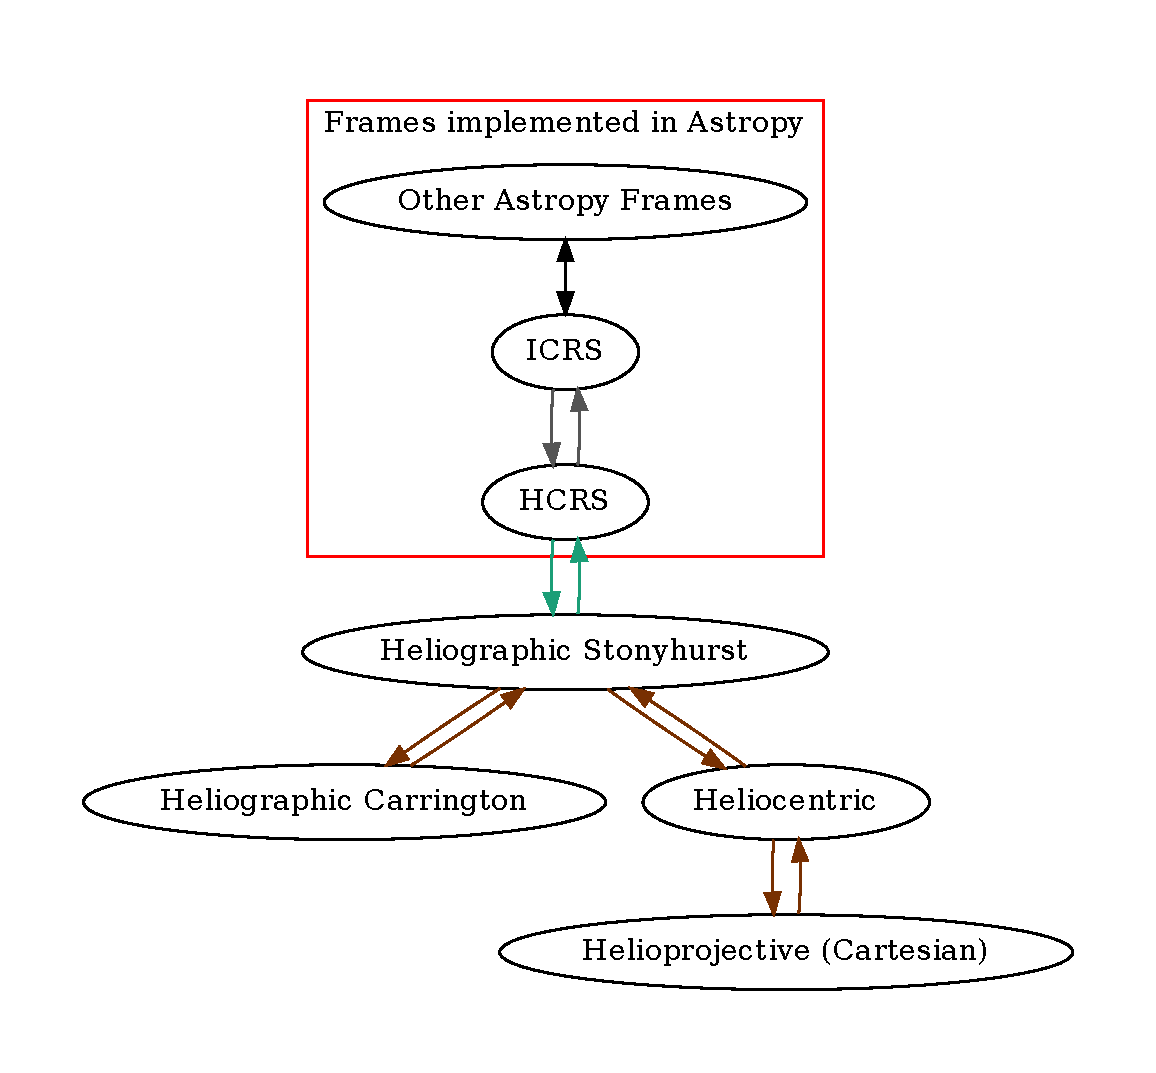
\includegraphics[width=0.75\textwidth]{figures/sunpy_frames.pdf}
    \caption{Graph of possible transformations between reference frames as implemented in \package{sunpy.coordinates}.
    The arrows indicate transformations between the different frames.
    Note that coordinates can be transformed to more general astronomical coordinate frames via the \hgs frame.}
    \label{fig:transform_graph}
\end{figure}

The observer-dependent coordinate frames -- HCC and HPC -- are useful for observational data, with the potential for subsequent transformation to an observer-independent frame.
The HPC frame in particular is widely used for images from solar missions.
These frames have axes that change orientation depending on the location of the observer, and thus the observer location is necessary to fully define the frame.
This observer location is also stored in the \code{SkyCoord} object.
If the observer is not explicitly specified, the observer is assumed to be at Earth, which may be a sufficient approximation for most observations.
Be aware that on the default observer of Earth does not fully define the frame unless the observation time is specified, since the location of Earth needs to be known.

The \package{sunpy.coordinates} subpackage enables significant functionality in the \sunpycode{Map} object (see \autoref{sec:map}), and a few examples are shown in \autoref{fig:coordinates_examples}.

\todo{brief description of figures}

\begin{figure}
    \gridline{\fig{figures/fieldlines_aia.pdf}{0.3\textwidth}{(a)}
              \fig{figures/fig_venus_transit.pdf}{0.3\textwidth}{(b)}
              \fig{figures/fig_coronagraph_starfield.pdf}{0.3\textwidth}{(c)}
              }
    \caption{Several example use cases of the coordinates machinery in \sunpy.
    (a) Field lines traced from a field extrapolation of active region NOAA XXXX computed using \package{pfsspy} overlaid on an 171 \AA image from AIA.
    (b) The Venus transit as viewed by SDO/AIA in 1600 \AA. The predicted position of Venus is overplotted in helioprojective coordinates of the AIA image.
    (c) A coronagraph image of the solar corona as observed by STEREO-A COR-2. The predicted positions of the stars from the Gaia DR2 catalog and mars are overplotted.}
    \label{fig:coordinates_examples}
\end{figure}

The above examples make use of functions in \package{sunpy.coordinates} to obtain the location of solar-system bodies.
\code{get\_body\_heliographic\_stonyhurst} not only returns the location of one of the planets, but can appropriately correct for light travel time to an observer to return the apparent location (in the past) of that planet.
This planet location is obtained using the active ephemeris in \package{astropy.coordinates}, so if one wants the location of a non-Earth body and accuracy is important, one should use \code{astropy.coordinates.solar\_system\_ephemeris} to specify a JPL ephemeris rather than Astropy's default ephemeris.
\code{get\_horizons\_coord} allows one to query JPL HORIZONS\footnote{\url{https://ssd.jpl.nasa.gov/?horizon}} for the location of a wide range of solar-system bodies.
JPL HORIZONS includes ephemeris information not only for planets and other natural bodies in the solar system, but also for major spacecraft such as SDO and SOHO.
This function requires the \package{astroquery}\footnote{\url{https://astroquery.readthedocs.io/en/latest/}} package to be installed and an Internet connection.

The coordinate framework is also used to calculate Sun-specific coordinate information with high accuracy.
These functions are under \package{sunpy.coordinates.sun} and return values such as Carrington rotation number for the provided time.
Nearly all of the returned values match values in the \textit{Astronomical Almanac} to published precision (e.g., the hundredth of an arcsecond for apparent right ascension).
For times that are provided to these functions, one should take care to specify whether the time scale is UT or some other time scale (e.g., TT).

\subsection{Solar differential coordination - Jack}

\todo{This section}
One paragraph long.
Not clear if it needs to be in this location.
Should it be in a map utility section?

Don't forget to refer to the figure!
An important application of....
Figure \ref{fig:diff_rot}


\begin{figure}
    \center
    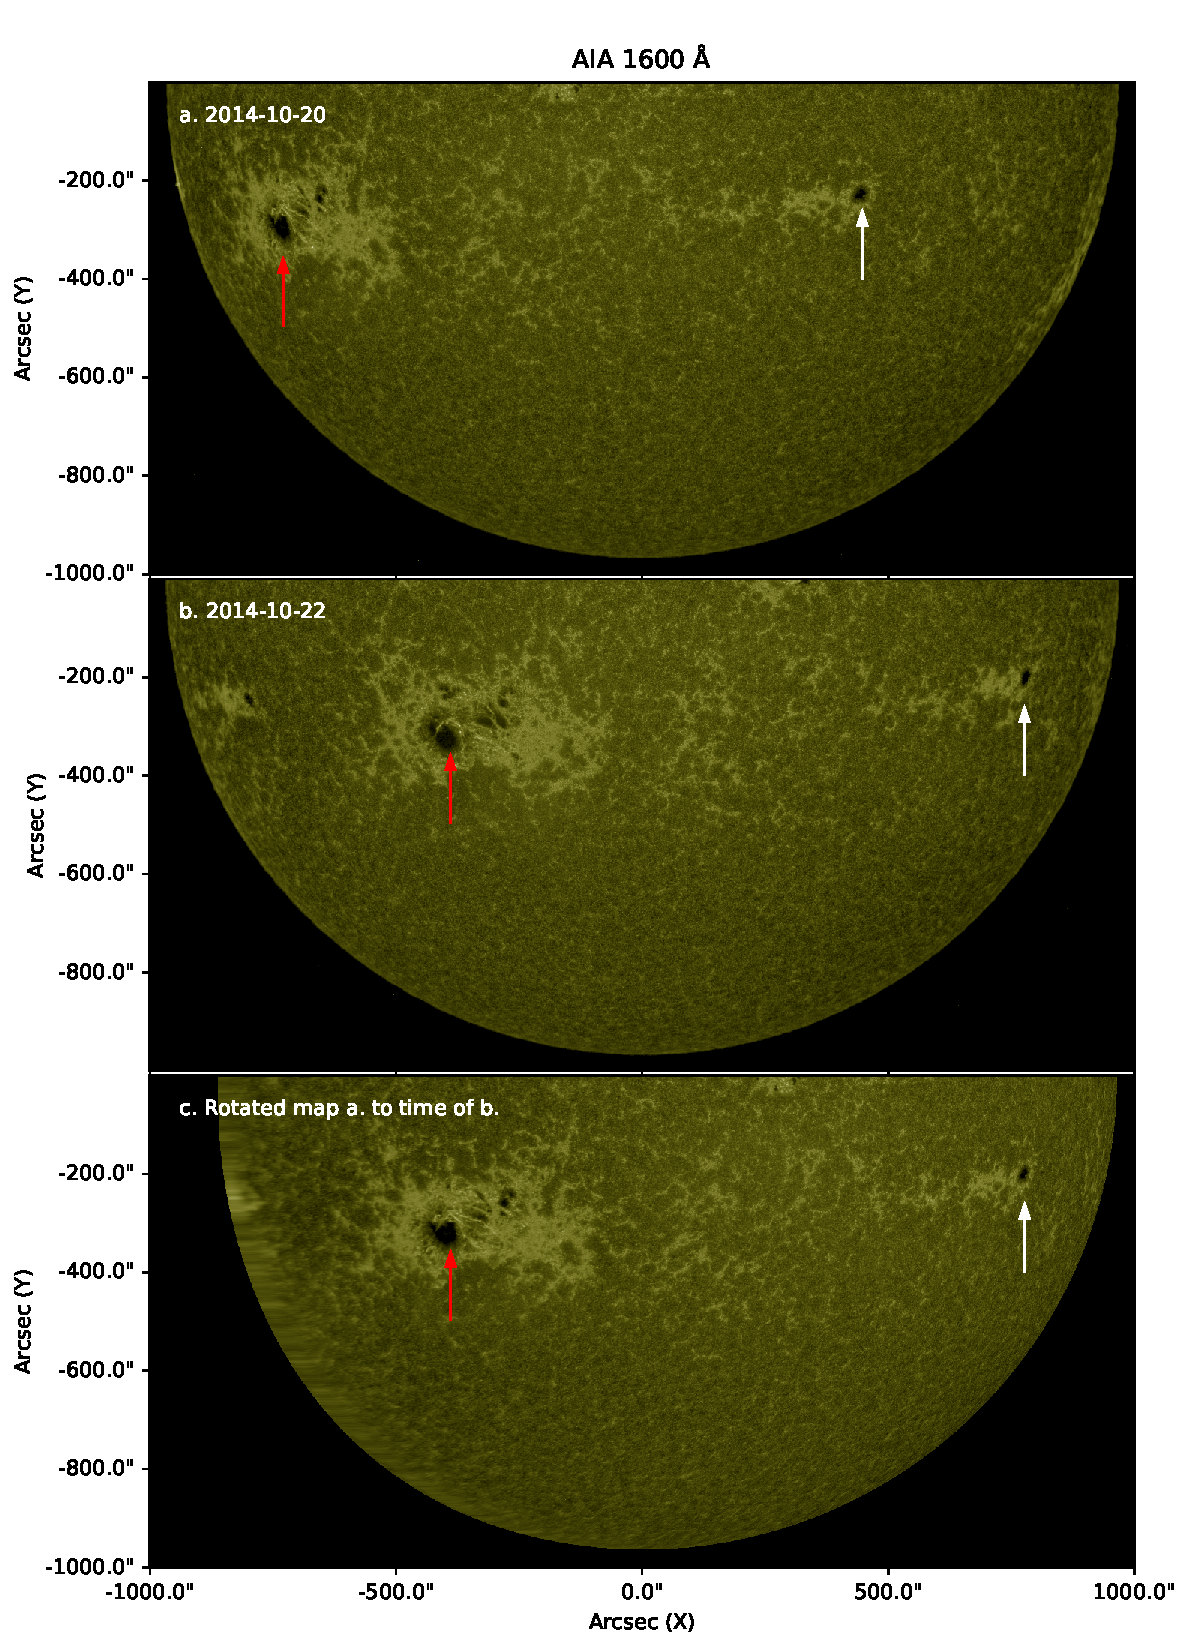
\includegraphics[width = 0.8\textwidth]{figures/diff_rot_1600.pdf}
    \caption{Example of the functionality of \sunpy to apply solar differential rotation to a Map.
    Panels (a) and (b) show the Sun as observed in AIA 1600~\AA\ on two different days, 2014-02-20 and 2014-02-22.
    A large sunspot group is highlighted by the red arrow, and a smaller sunspot by the white arrow.
    Panel (c) shows the map of (a) that has been rotated differentially using \sunpy to the time of map (b).}
    \label{fig:diff_rot}
\end{figure}
